\section{Технические средства моделирования}

\textbf{Использование}

\begin{itemize}
    \item Используются как средства расчета по полученным моделям
    \item Используются как средства имитационного моделирования
\end{itemize}

\textbf{Средста}

\subsection{Цифровая вычислительная техника}

\textbf{Центральный процессор} -- выполнение арифметико-логических операций и дешифрация и обработка команд.

\textbf{Память} -- электро-механическое устройство, предназначенное для записи, хранения и выдачи информации.

\subsection{Аналоговая вычислительная техника}

В отличие от дискретной, в основе аналоговой вычислительной техники заложен принцип моделирования при использовании в качестве моделей электронных цепей, каждой переменной величине задачи ставится соответствие переменная величина электронной цепи. При этом основой построения такой модели является изоморфизм (подобие исследуемой задачи и соответствующей ей электронной модели). В большинстве случаев при определении критериев подобия используются специальые приемы \textbf{масштабирования} соответствующих значений параметра модели и переменных задач. АВМ реулизует модели изоморфную исследуемой заадчи. Согласно своим вычислительным возможностям АВМ, приспособленное для исследования объектов, динамика которых описывается обыкновенными и в частных производных дифферинциальными уравнениями.

Под АВМ будем понимать совокупность электрических элементов, организованных в систему, позволяющую изоморфно моделировать динамику изучаемого объекта, Функциональные блоки АВМ должны реализовывать весь комплекс арифметико-логических операций.

АВМ делятся по мощности:

\begin{itemize}
    \item малые ($n < 10$)
    \item средние ($10 \le n \le 20$)
    \item большие аналоговые комплексы ($n \geq 20$)
\end{itemize}

\subsection{Гибридная вычислительная техника}

\begin{figure}[H]
    \centering
    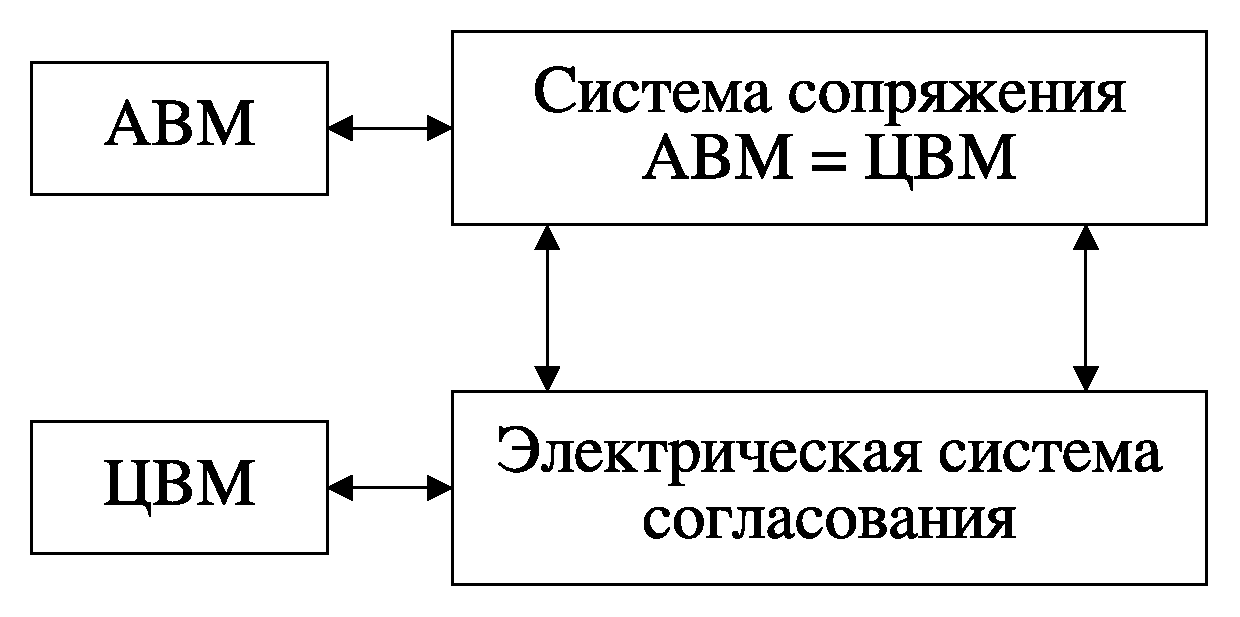
\includegraphics[width=0.8\textwidth]{img/content/04_technical/hybrid.pdf}
    \caption{Гибридная ВМ}
    \label{fig:hybrid}
\end{figure}

В общем случае под гибридной ВМ понимается широкий класс технических устройств, использующих как аналоговую, так и дискретную форму представления и обработки информации.

\subsubsection{Подклассы АВМ}

\begin{enumerate}
    \item АВМ, использующие численные методы анализа.
    \item АВМ, программируемые с помощью ЦВМ.
    \item АВМ с цифровым управлением и логикой.
    \item АВМ с цифровыми элементами.
    \item ЦВМ с аналоговыми арифметическими устройствами.
    \item ЦВМ, допускающее программирование аналогово типа.
\end{enumerate}
